\documentclass[10pt,twocolumn,letterpaper]{article}

\usepackage{icb}
\usepackage{times}
\usepackage{epsfig}
\usepackage{graphicx}
\usepackage{amsmath}
\usepackage{amssymb}
\usepackage{eso-pic}

% Include other packages here, before hyperref.

% If you comment hyperref and then uncomment it, you should delete
% egpaper.aux before re-running latex.  (Or just hit 'q' on the first latex
% run, let it finish, and you should be clear).
%\usepackage[pagebackref=true,breaklinks=true,letterpaper=true,colorlinks,bookmarks=false]{hyperref}

\icbfinalcopy % *** Uncomment this line for the final submission

\def\icbPaperID{****} % *** Enter the IJCB Paper ID here
\def\httilde{\mbox{\tt\raisebox{-.5ex}{\symbol{126}}}}

% Pages are numbered in submission mode, and unnumbered in camera-ready
\ificbfinal\pagestyle{empty}\fi
\begin{document}

%%%%%%%%% TITLE
\title{Investigation of muscular architecture in ultrasound images}

\author{Thomas Bergmueller, Martin Schnoell\\
Medical Imaging LAB\\
Master program: Applied Image and Signal Processing\\
Fachhochschule Salzburg\\
%Institution1 address\\
{\tt\small tbergmueller.aise-m2013@fh-salzburg.ac.at, mschnoell.aise-m2013@fh-salzburg.ac.at}
% For a paper whose authors are all at the same institution,
% omit the following lines up until the closing ``}''.
% Additional authors and addresses can be added with ``\and'',
% just like the second author.
% To save space, use either the email address or home page, not both
%\and
%Second Author\\
%Institution2\\
%First line of institution2 address\\
%{\tt\small secondauthor@i2.org}
}

\maketitle
\thispagestyle{empty}

%%%%%%%%% ABSTRACT
%\begin{abstract}
%   The ABSTRACT is to be in fully-justified italicized text, at the top
%   of the left-hand column, below the author and affiliation
%   information. Use the word ``Abstract'' as the title, in 12-point
%   Times, boldface type, centered relative to the column, initially
%   capitalized. The abstract is to be in 10-point, single-spaced type.
%   Leave two blank lines after the Abstract, then begin the main text.
%   Look at previous ICB abstracts to get a feel for style and length.
%\end{abstract}

%%%%%%%%% BODY TEXT

\section{Introduction}
The main goal of this project was to write an algorithm which automatically calculates the angle between the aponeurosis and the muscle fibers of the Vastus Lateralis which is the muscle on the thigh right over the knee. This angle correlates with the constitution of the muscle.
For this project we used ultrasound images.  
Figure \ref{fig:VastusLateralis} shows the location of the Vastus Lateralis and an example ultrasound image in which both aponeuroses (lower and upper one) as well as the line is drawn which represents the muscle fibers (dashed line). Between this muscle fibers and the aponeurosis the angle should be calculated. In the most cases, the two aponeuroses are parallel, so there is no difference between taking the upper or lower one for the calculations. However, sometimes the two aponeuroses are not parallel and then, usually, the lower one is used. 


\begin{figure}
	\begin{center}		
		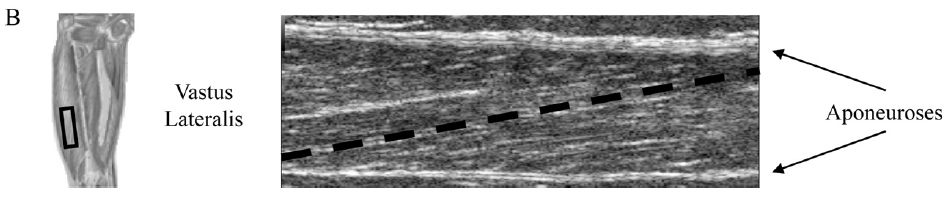
\includegraphics[width=1\linewidth]{img/VastusLateralis}
	\end{center}
	\caption{Vastus Lateralis (left) and an example ultrasound image in which both aponeuroses (lower and upper one) as well as the line is drawn which represents the muscle fibers (dashed line). \cite{NCronin13a}}
	\label{fig:VastusLateralis}
	
\end{figure}

Usually, this angle is calculated manually, by fitting lines to an ultrasound image on the computer and then calculate the angle by hand.

The available groundtruth consists of 22 ultrasound images of the Vastus Lateralis from 12 different patients.
Figure \ref{fig:im1_orig} shows one original image of the dataset.

\begin{figure}
	\begin{center}		
		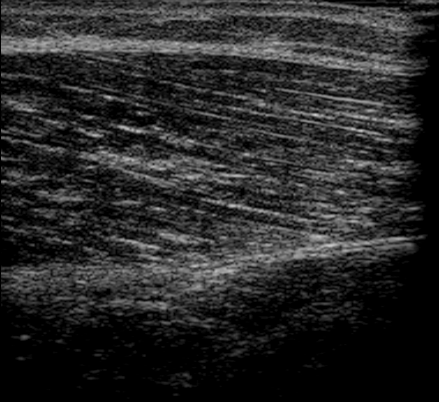
\includegraphics[width=1\linewidth]{img/im1_original}
	\end{center}
	\caption{One original image of the dataset.}
	\label{fig:im1_orig}
	
\end{figure}

For every image two or three different measurements of the angle exist, which partly vary significantly. For example, is the biggest difference of two measurements for the same image (!) 5.7 degree (image with ID 1). In the most cases, however, the single measurements are in the range of +/- 1.5 to the mean.
For our implementation we calculated the mean angle of all measurements from one image and took this mean angle as a reference.

\section{Proposed algorithms}
We worked on two different algorithms in order to determine the angle. The first one is the Hough transform, which is a well-known algorithm for detecting lines in an image \cite{c1962method}. The second one is based on template matching.

\subsection{Hough transform}
\label{sec:hough}
The Hough transform is a well-known and established algorithm for detecting lines and other shapes in images. For the implementation, we used MATLAB R2013a and the inbuilt MATLAB function hough.
This are the main steps of our implementation:

\begin{enumerate}
     \item Gamma correction for enhancing the white pixels
     \item Binarization of the image
     \item Hough transform applied directly on the binary image in order to detect the aponeurosis (the most prominent line)
     \item Canny edge detection on the binary image
     \item Hough transform on the edge image
     \item Finally: Calculate the mean angle of all muscle fiber candidates and then determine the difference between the angle of the aponeurosis and the mean. This results in the final angle
\end{enumerate}

For detecting the aponeurosis (step 3) we also restricted the hough function to only search for lines which are nearly horizontal ( +/- 10 degree roughly). This increases the probability for finding the correct aponeurosis. In step 6, finding the muscle fiber candidates means that the 25 most prominent lines are used. Here, the angle is also restricted to the range from ~6 to ~30 degree since almost all muscle fibers in the groundtruth are in this range and lines with other angles are then clearly outliers. Furthermore, depending on the position of the aponeurosis (at the top or bottom), the fiber candidates have to clearly also lay below (detected aponeurosis is at the top) or above (apo. at bottom) the aponeurosis.

Figure \ref{fig:im1_hough_apo} shows the detected aponeurosis and \ref{fig:im1_hough_fibers} shows the muscle fiber candidates on the image with ID 1 of the database.

\begin{figure}
	\begin{center}		
		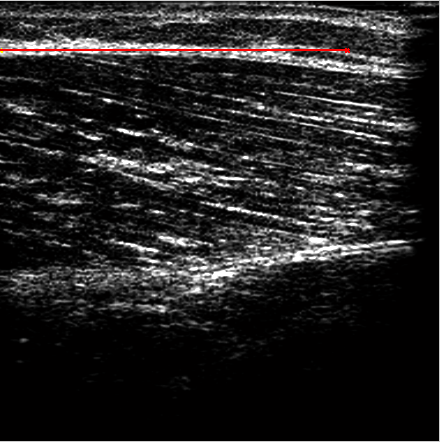
\includegraphics[width=0.7\linewidth]{img/im1_hough_apo}
	\end{center}
	\caption{This image shows the detected aponeurosis (red line) of the hough transform approach.}
	\label{fig:im1_hough_apo}
	
\end{figure}

\begin{figure}
	\begin{center}		
		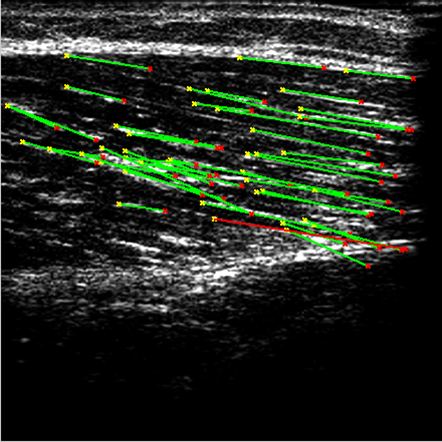
\includegraphics[width=0.7\linewidth]{img/im1_hough_fibers}
	\end{center}
	\caption{This image shows the 25 detected muscle fiber candidates from which the mean angle is taken.}
	\label{fig:im1_hough_fibers}
	
\end{figure}

\subsection{Template Matching - a proof of concept}
As a second approach we introduce a method based on template matching. In template matching anything that serves as a model can be used to compute the similarity to a second instance of this model \cite{Brunelli09a}. The basic idea behind our template approach is that we can obtain the fascicle angle by moving around probe regions of the original image in a local neighbourhood of the probe location. Because we assume fascicles can be seen as straight lines - at least locally - the similarity reaches a maximum for movements along that line. Hence, by detecting which specific movements result in maximum similarity between probe region and a sample-region of equal size within it's local neighbourhood, we are going to detect the fascicle angle.


We take a rectangular sample region and compute similarity scores within a probe region. This process is illustrated in figure \ref{fig:templateApproach}. 

\begin{figure}
	\begin{center}		
		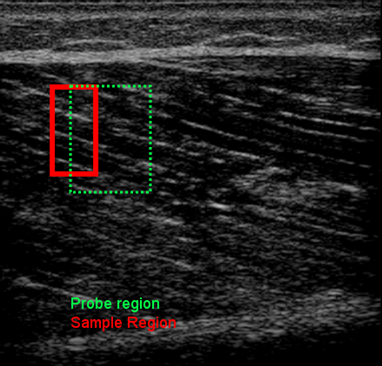
\includegraphics[width=0.7\linewidth]{img/templateApproach}
	\end{center}
	\caption{In the template approach a rectangular sample region (red) is extracted from the image. Then the sample is moved around within the probe region (green) and for each possible position the similarity score is computed.}
	\label{fig:templateApproach}
	
\end{figure}

As a similarity score we employ the pixel-wise absolute difference between each pixel in the probe region and the corresponding pixels of a sub-region (same size as the probe region) within the sample region.

\begin{figure}
	\begin{center}		
		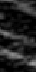
\includegraphics[width=0.09\linewidth]{img/sample}
		\hspace{0.05\linewidth}
		
\includegraphics[width=0.2\linewidth]{img/diff1}
		
\includegraphics[width=0.2\linewidth]{img/diff2}
		
\includegraphics[width=0.2\linewidth]{img/diff3}
		
\includegraphics[width=0.2\linewidth]{img/diff4}
	\end{center}
	\caption{Left the sample region (red in fig. \ref{fig:templateApproach}) is shown and to the right four similarity maps (green in fig. \ref{fig:templateApproach}) from different probe regions. In the similarity maps, black indicates high similarity, while white means no similarity at all. }
	\label{fig:sampleAndSimScores}
\end{figure}

In doing so, for each sample region a similarity score map is computed. Such sample similarity score maps are shown in figure \ref{fig:sampleAndSimScores}. From the sample regions in figure \ref{fig:sampleAndSimScores} an intuitive proof of the template approach is seen. Especially the first and fourth similarity map have the highest similarities arranged in a straight line. This proofs the assumption that moving the sample region along a straight line in direction of the fascicles always results in maximum similarity. By finding the position of maximum similarity within the similarity maps, the fascicle angle can be computed. We define $P_{max}$ as the position of the maximum similarity within the similarity map, $P_P$ the upper left corner of a probe region with width $w_P$ and height $h_P$. The system is configured to have the upper left corner of the sample region $P_S$ at 
\begin{equation}
P_S=(P_{P_x}+\frac{1}{2}w_P, P_{P_y}).
\end{equation}

This works under the assumption that the fascicle orientation is always towards the lower right corner of the image, hence in increasing x- and y-direction\footnote{The origin is at the upper left corner of the image}. 

Therefore, we can define a direction vector V that defines is parallel to the fascicles by using $P_max$ and $P_P$. By computing the angle of this vector we get the fascicle orientation $\phi_{P_P}$ at a probe location $P_P$ as

\begin{equation}
\phi_{P_P} = arctan(\frac{(P_{max_y} + P_{S_y}) - P_{S_y}}{(P_{max_x} + P_{S_x}) - P_{S_x}})
\end{equation}

Now, this fascicle orientation $\phi_{P_P}$ represents the local orientation around a probe point $P_P$. Because - as can be seen from the testing data - fascicles are not necessarily straight lines throughout the whole ultrasound image. To account for this, we compute a angle field, which is shown in blue in figure \ref{fig:angleField} by computing the local fascicle orientation for multiple probe points.

\begin{figure}
	\begin{center}		
		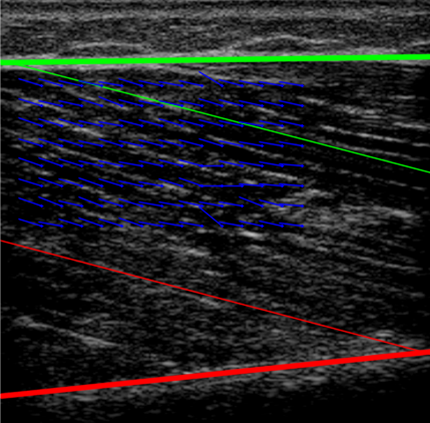
\includegraphics[width=0.7\linewidth]{img/angleField}
	\end{center}
	\caption{The detected upper (thick green) and lower (thick red) aponeuroses as well as the angle field (blue). Furthermore, the thin red and green line represent the mean fascicle orientation $\overline{\phi_{P_P}}$ }
	\label{fig:angleField}
	
\end{figure}

As can be seen from figure \ref{fig:angleField}, there are sometimes false angles detected for certain probe points $P_P$. To limit the impact of such errors, the mean fascicle angle $\overline{\phi_{P_P}}$ over the angle field is computed by simply taking the arithmetic average of all local fascicle angles. The mean fascicle angle is illustrated in figure \ref{fig:angleField} as a thin red and green line.

Finally, as described in section \ref{sec:hough}, the mean fascicle angle is related to the angle of upper (green) and lower (red) aponeurosis. Since we have no clear evidence which is the correct aponeurosis for this procedure, we decided to compute both relative fascicle angles and label them accordingly.  

\subsection{A more elaborate method to find upper and lower aponeuroses}
\label{sec:apofinding}
As described, Hough Lines are used for detection of the aponeuroses. In most of our testing data, two aponeuroses, subsequently denoted as upper- and lower aponeurosis, are pictured. Hence an algorithm has to be found to determine upper- and lower aponeuroses. We propose (considering the line equation $y = kx +d $):

\begin{enumerate}
	\item Find all possible candidates
	\item Robustly group parallel lines according to $k \pm \Delta k$
	\item For each $k$-group, group members to d-groups according to $d \pm \Delta d$.
	\item Upper Aponeuroses: The mean line of the most-upper d-group.
	\item Lower Aponeuroses: The mean line of the most-lower d-group  
	\item Detection criteria: Upper Apo must be in upper half of the ultrasound image, lower Apo must be below the center line of the ultrasound image. 
\end{enumerate}

This works intuitively well, as evaluated experimentally with our 22 sample images. The lower aponeuroses is illustrated as a thick red line in figure \ref{fig:angleField} whereas the upper aponeuroses is ullustrated as a thick green line.





\section{Results}
The average error and distance to the groundtruth values for all 22 images of both approaches is as following: 

\begin{itemize}
     \item \emph{Hough transform}: \textbf{2.48 degree}
     \item \emph{Template matching}: \textbf{2.75 degree}
\end{itemize}

What has to be clearly considered, is the fact that the angles in the groundtruth are measured quite differently. So, if the groundtruth would have been constructed uniformly (with uniform ways of measuring the angle), we suppose that the results of our approaches would result in an even lower error.


\subsection{Discussion of Hough transform results}

With an average error of 2.48 degree the Hough transform performs overall really well and outperforms the template matching results. 
However, improvements could be clearly done in the aponeurosis detection since in the most cases the detected aponeurosis is just a purely horizontal line which a user would in some cases clearly not agree with. An example of such a situation can be seen in Figure \ref{fig:im7_hough_apo}. Here, the left part of the aponeurosis is clearly not horizontal, although this is the case on the right part. However, the user would expect that the detected line is closer to the left part of the aponeurosis.
The muscle fibers are giving in general really good results, so the strategy of taking 25 fiber candidates and average them in order to find the angle clearly pays off.

\begin{figure}
	\begin{center}		
		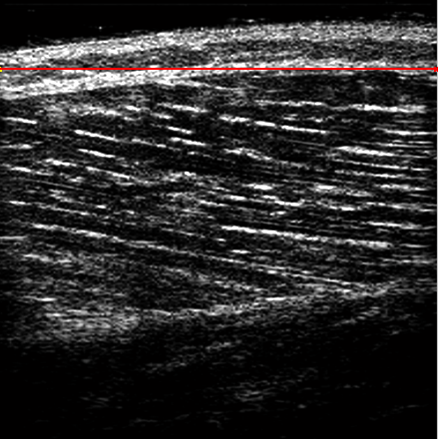
\includegraphics[width=0.45\linewidth]{img/im7_hough_apo}
		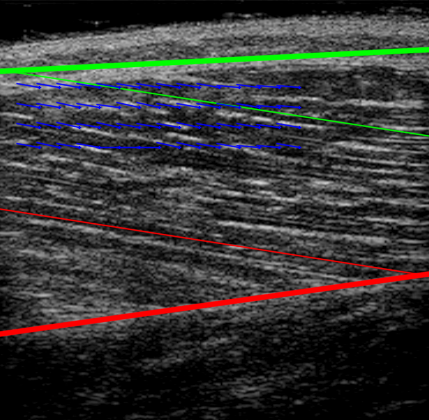
\includegraphics[width=0.45\linewidth]{img/im7_apo_ela}
	\end{center}
	\caption{Detected aponeurosis of image 7 with the standard houghline-approach (left) vs. detected upper and lower aponeuroses (right) with the method described in section \ref{sec:apofinding}  .}
	\label{fig:im7_hough_apo}
	
\end{figure}

\subsection{Discussion of template matching results}
In comparison to the hough transform approach, the template matching approach performs in average similar. However, when looking at individual results some remarks have to be made. It is still not clear whether the angle between lower- or upper aponeurosis is the measured angle in the ground truth. For rating (refer table \ref{tab:results}), in the template matching approach the angle to the lower aponeurosis is used (if available). If the lower aponeurosis can't be detected, the angle to the upper aponeursis is used. In some cases, as for instance shown for image 7 in figure \ref{fig:im7_hough_apo}, the template matching approach outperforms the hough-lines because of the more accurate aponeuroses detection. 

\begin{figure}
	\begin{center}		
		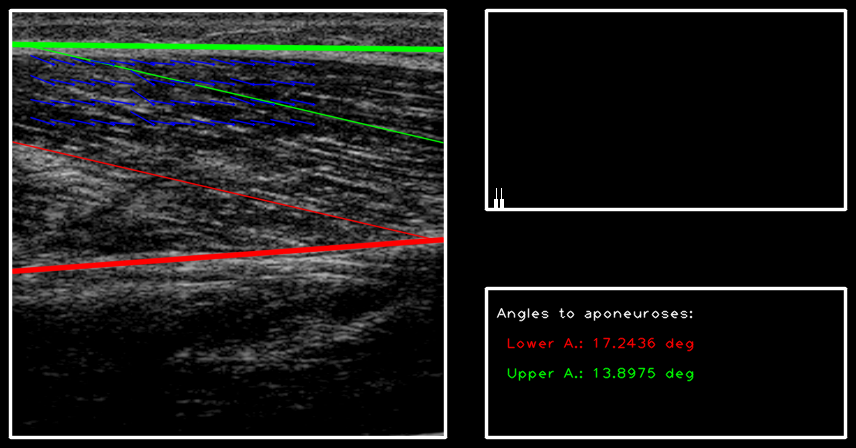
\includegraphics[width=\linewidth]{img/im2_resView_tm}
		
	\end{center}
	\caption{Complete result view of image 2 examination with the template matching approach. To the left, the visualization of found features, to the right the histogram of local fascicle angles and the angle between mean fascicle angle and upper respectively lower aponeurosis.}
	\label{fig:im2_results}
\end{figure}

The field of local fascicle angles shows significant variation in the angles, as pictured in the histogram of figure \ref{fig:im2_results}. This is mostly due to a absolute minimum detection for the probe region moving vector, which is by nature prone to noise. Furthermore, at the moment only a arithmetic mean over all local fascicle angles is used to come up with the mean fascicle orientation. As can be seen from the histogram in figure \ref{fig:im2_results} as well, there might be a bimodal histogram, where the mean angle lies somewhere were no angle has ever been detected. Here a more elaborate approach might be helpful as well.

In general, there are several weaknesses due to only being proof-of-concept and no beta version implementation. These are listed in section \ref{sec:future}.

\subsection{Comparison of both approaches}

Table \ref{tab:results} shows the groundtruth angles as well as the angles from both approaches for every single image.
Figure \ref{fig:errorPlot} shows an error plot of both strategies. As it can be seen in the plot, both algorithms do not always agree on a low or high distance to the groundtruth. So for some images like images 5, 19 and 20 the Hough transform clearly beats the template matching approach where e.g. for images 7 and 14 the template matching result is clearly the better one.
Image 15 is clearly the most challenging one and the corresponding groundtruth image (the image where the lines are drawn by hand from an expert user) is shown in Figure \ref{fig:im15_gt}. 
The hand-drawn lines are looking correct, although it can be seen that the original muscle fibers have some curvature, so the hand-drawn three fiber lines can clearly not cover such a curvature and represent more the left part of the fibers.
Figure \ref{fig:im15_hough_apo} and \ref{fig:im15_hough_fibers} are showing the Hough transform results and figure \ref{fig:im15_templ} the template matching results.
Both approaches seem to detect the correct lines and angles when looking at the corresponding images. So at least, both strategies cannot be considered as completely faulty in this case and it might be the case that just the groundtruth angle is not correct or is too far away from the really "true" angle.

\begin{figure}
	\begin{center}		
		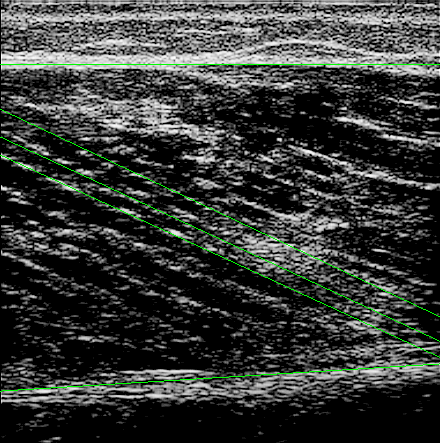
\includegraphics[width=0.47\linewidth]{img/im15_gt}
		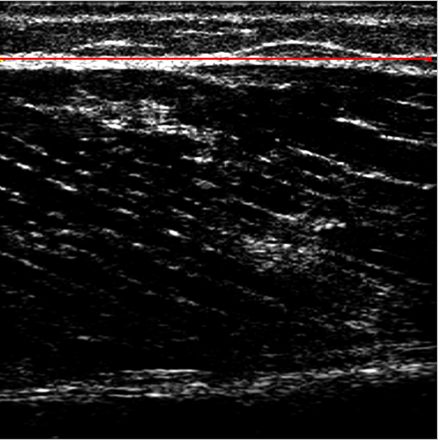
\includegraphics[width=0.47\linewidth]{img/im15_hough_apo}
	\end{center}
	\caption{Image 15 and the corresponding groundtruth lines (left) as well as the detected aponeurosis with the standard approach (right)}
	\label{fig:im15_gt}
	
\end{figure}



\begin{figure}
	\begin{center}		
		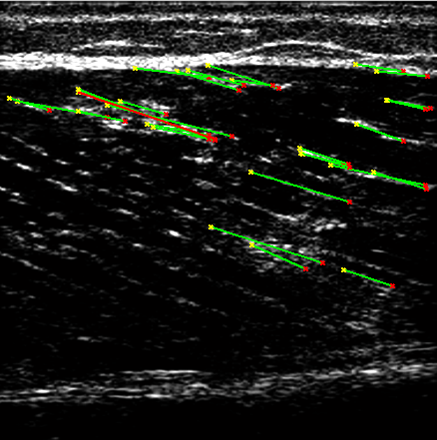
\includegraphics[width=0.47\linewidth]{img/im15_hough_fibers}
		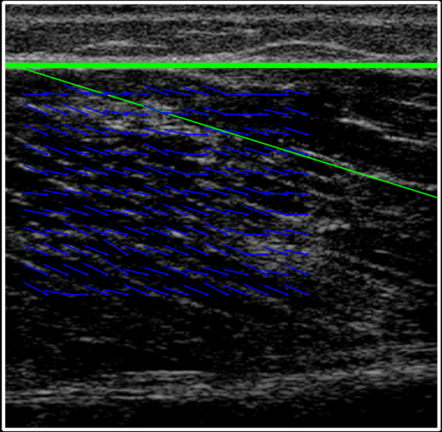
\includegraphics[width=0.47\linewidth]{img/im15_templ}
	\end{center}
	\caption{Image 15 and the detected fiber candidates from the Hough transform approach (left). The results of the template matching approach are pictured right.}
	\label{fig:im15_hough_fibers}	
\end{figure}



\begin{table}
\begin{center}
\begin{tabular}{| l | l | l | l |}
  \hline
  \emph{Image ID} & \emph{GT} & \emph{HT} & \emph{TM} \\ \hline
  1 & 13.73 & 12.82 & 18.43 \\ \hline
  2 & 16.07 & 13.39 & 17.24 \\ \hline
  3 & 11.70 & 13.34 & 10.56 \\ \hline
  4 & 12.00 & 13.53 & 11.50 \\ \hline
  5 & 13.55 & 10.64 & 7.10 \\ \hline
  6 & 11.60 & 14 & -666 \\ \hline
  7 & 17.20 & 11.34 & 16.83 \\ \hline
  8 & 10.63 & 12.27 & 12.32 \\ \hline
  9 & 11.17 & 11.16 & 8.49 \\ \hline
  10 & 16.47 & 10.86 & 11.19 \\ \hline
  11 & 12.10 & 11.93 & 15.12 \\ \hline
  12 & 13.35 & 13.56 & 11.90 \\ \hline
  13 & 13.57 & 15.09 & 11.65 \\ \hline
  14 & 19.50 & 14.67 & 20.56 \\ \hline
  15 & 24.90 & 14.57 & 17.35 \\ \hline
  16 & 13.23 & 12.87 & 9.59 \\ \hline
  17 & 14.20 & 12.57 & 12.90 \\ \hline
  18 & 13.75 & 12.66 & 9.03 \\ \hline
  19 & 17.30 & 13.83 & 9.42 \\ \hline
  20 & 17.97 & 14.66 & 11.63 \\ \hline
  21 & 10.37 & 11.73 & 9.51 \\ \hline
  22 & 12.30 & 11.19 & 13.49 \\ \hline
\end{tabular}
\caption{Comparison of the angles from the groundtruth (GT), the hough transform approach (GT) and from the template matching approach (TM).}
\label{tab:results}
\end{center}
\end{table}

\begin{figure}
	\begin{center}		
		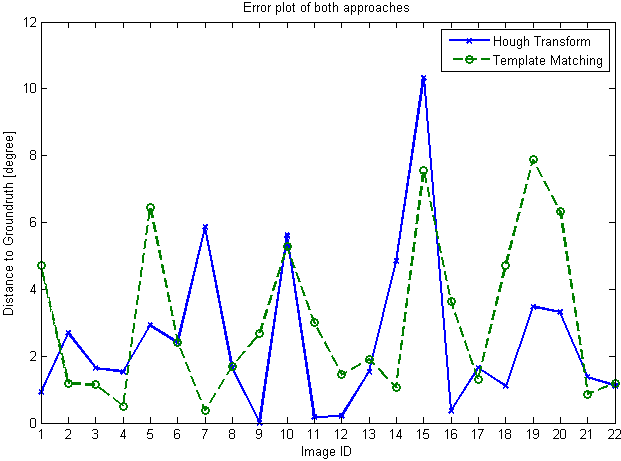
\includegraphics[width=1\linewidth]{img/ErrorPlot2}
	\end{center}
	\caption{Error plot of both approaches.}
	\label{fig:errorPlot}
	
\end{figure}


\section{Conclusion}
Both strategies gave good results when looking at the distances to the groundtruth angles. Clearly, with a bigger and more reliable groundtruth both algorithms could be even more optimized.

\section{Future work}
\label{sec:future}
Especially for the template matching approach only a proof-of-concept has been brought. Therefore there's huge potential for improvement. We like to note the most promising one briefly:

\begin{itemize}
	\item Histogram approach to find mean fascicle orientation
	\item Even the median might work better here
	\item Do not only take the distance minimum to come up with the maximum similarity during template matching, but try line fitting approaches throughout the local fascicle angle maps.
	\item Template matching is weak when there is no clear fascicle line visible in the image, that is when the probe region is either black or white or gray. This can be avoided by ruling out images with such characteristics. A good start would be using thresholding on standard deviation or mean gray values.
\end{itemize}
	

{\small
\bibliographystyle{ieee}
\bibliography{egbib}
}

\end{document}
